\documentclass[12pt,a4paper]{amsart}

\usepackage[slovene]{babel}
\usepackage[utf8]{inputenc}
\usepackage{amsmath,amssymb,amsfonts}
\usepackage{url}
\usepackage[dvipsnames,usenames]{color}
\usepackage{graphicx}
\graphicspath{ {images/} }
 
%\usepackage{xparse}

\textwidth 15cm
\textheight 24cm
\oddsidemargin.5cm
\evensidemargin.5cm
\topmargin-5mm
\addtolength{\footskip}{10pt}
\pagestyle{plain}
\overfullrule=15pt 


\newcommand{\program}{Finančna matematika}

\newcommand{\naslovdela}{Problem največjega polnega podgrafa}
\newcommand{\imeavtorja}{Vida Maver, Anamarija Mijatović}


\theoremstyle{definition}
\newtheorem{definicija}{Definicija}[section]
\theoremstyle{plain}
\newtheorem{trditev}[definicija]{Definicija}

\begin{document}

\begin{center}{\large
\vspace*{\fill}
{\bf \LARGE{\naslovdela}}\\[10mm]}

\textbf{Poročilo}

\textbf{Predmet:} Finančni praktikum
\\
\textbf{Avtorici:}\imeavtorja\\[2mm]

\center{5.1.2018}
\vspace*{\fill}
\end{center}
\pagebreak


\tableofcontents

\pagebreak

\section{Kratek opis problema}

V svojem projektu sva se ukvarjali z optimizacijskim problemom iskanja 
največjega polnega podgrafa na nausmerjenih grafih, oziroma povedano drugače, s problemom iskanja maksimalne klike v danem neusmerjenem grafu. \\

Klika je podgraf grafa, v katerem so vsa vozlišča med seboj sosednja. 
Polni graf reda $n$ je graf z $n$ vozlišči, v katerem obstaja povezava med vsakim parom različnih vozlišč. Označimo ga s $K_n$, v njem pa je $\frac{n(n - 1)}{2}$ povezav. 
Največja klika (ang. \textit{maximal}) $C$ na neusmerjenem grafu G je polni podgraf, ki ni vsebovan v nobenem drugem polnem podgrafu, torej če ne obstaja klika $C'$ na grafu $G$, tako da $C$ $\subseteq$ C' in C $\ne$ C'. 
Naj bo V množica vozlišč grafa $G(V, E)$. Polni podgraf grafa $G$ je taka množica $G'$ $\subset$ $G$, da za vsak par vozlišč $v, w$ $\in$ $V$, kjer $v$ $\ne$ $w$, velja, da sta na grafu $G$ sosednja. 
Poznamo tudi pojem maksimalne klike. Kliki $C_{max}$ rečemo maksimalna (ang. \textit{maximum}) klika, če ne obstaja klika na grafu $G$, ki bi vsebovala več vozlišč. 
Število vozlišč v maksimalni kliki označimo z $\omega(G)$ in ga imenujemo klično število. Velja, da je vsaka maksimalna klika $C_{max} \subseteq V$ na grafu $G$ največja klika, obratno pa ni nujno res. Na primeru si oglejmo kliko in maksimalno kliko:

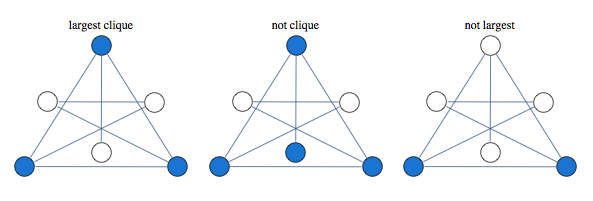
\includegraphics[width=\textwidth]{cliques}

Iskanje maksimalne klike na neusmerjenem grafu je eden od pomembnih NP - težkih problemov, uporablja pa se predvsem v diskretni matematiki, bioinformatiki in računalniški kemiji. Problem je NP - težek, če zanj ne obstajajo učinkoviti natančni polinomski algoritmi in se zato raje posvetimo iskanju algoritmov, ki v korist hitrosti žrtvujejo natančnost.\\

Največjo kliko bi lahko iskali s sistematičnim pregledom vseh podmnožic, vendar bi takšno iskanje vzelo preveč časa in ne bi bilo uporabno za grafe z večjim številom vozlišč. Poznamo pa algoritme, ki potrebujejo manj časa za reševanje problema. Med njimi sta Bron-Kerbosch algoritem in MaxClique algoritem, ki sta uporabna za iskanje največje klike na neusmerjenih grafih. Bron in Kerbosch sta leta 1973 predstavila algoritem za iskanje vseh klik na neusmerjenm grafu z uporabo metode "razveji in omeji". Pri tej metodi možne rešitve hranimo in ocenjujemo njihovo obetavnost. MaxClique algoritem pa najde maksimalno kliko grafa, ki je neke omejene velikosti in je v ta namen koristno poznati čimbolj natančne meje, zato je ideja algoritma za izračun največje klike na neusmerjenih grafih ta, da bi bile v začetku algoritma že izračunane tesne zgornje meje, kar močno skrajša čas, ki je potreben za rešitev problema.
\\

Za reševanje problema si torej lahko pomagamo z več formulacijami v celoštevilskem linearnem programiranju. Midve sva si pomagali s formulacijo za iskanje maksimalne neodvisne množice grafa $G$. Samo formulacijo bova opisali v nadaljevanju.\\

V kakšnih aplikacijah pa nas namesto klike oziroma polnega podgrafa zanima zgoščen podgraf (ang. \textit{dense subgraph}), za katerega velja, da je vsaj $(a*100)\%$, $0 \leq a \leq 1$  povezav, ki bi v kliki morale biti, že v njej.  Denimo, da imamo graf $G$ z $n$ vozlišči in zahtevano gostoto $a$. Potem lahko definiramo kliko, kvazikliko in k-psevdokliko. 
\\

\begin{itemize}
\item Klika velikosti $t$ je taka podmnožica $C$ vozlišč iz $G$ s $|C| = t$, da sta poljubni vozlišči iz $C$ sosednji v $G$, kar pomeni, da ima podgraf $G$, induciran na $C$, $\frac{t*(t-1)}{2}$ povezav.
\\

\item Kvaziklika velikosti $t$ je taka podmnožica $Q$ vozlišč iz $G$ s $|Q| = t$, da ima podgraf $G$, induciran na $Q$, vsaj $\frac{a*t*(t-1)}{2}$ povezav.
\\

\item $k$ - psevdoklika velikosti $t$ (za neko število $k$) je taka podmnožica $P$ vozlišč iz $G$ s $|P| = t$, da ima podgraf $G$, induciran na $P$, vsaj $\frac{a*t*(k-1)}{2}$ povezav.

\end{itemize}



\subsection{Časovna zahtevnost}
Če nas zanima, ali graf $G$ vsebuje kliko, ki ima $k$-vozlišč in če želimo najti vse take, lahko uporabimo tako imenovan \textit{brute force} algoritem. Tak algoritem preveri vsak podgraf grafa $G$, ki ima $k$ vozlišč in preveri če ta tvori kliko. Časovna zahtevnost tega postopka je $O(n^kk^2)$, ker mora algoritem preveriti $O(n^k)$ podgrafov, kjer pa mora nadalje še pri vsakem od teh preveriti $O(k^2)$ povezav. Vidimo, da je problem lahko rešen v polinomskem času, če je parameter $k$ fiksna konstanta, če pa temu ni tako, pa je časovna zahtevnost tega algoritma eksponentna.

Moon \& Moser pa sta ugotovila, da ima vsak graf z $n$ vozlišči največ $3^{n/3}$ maksimalnih klik.

\section{Postopek}
\subsection{Opis podatkov}

Ker je bila najina naloga uporabiti celoštevilsko linearno programiranje za iskanje maksimalnih klik v grafih, ki jih lahko najdemo na internetu, sva si v začetni fazi izbrali konkreten graf, na katerem sva kasneje delali. Za konkretni primer sva si izbrali glasovanje znotraj Wikipedijinga omrežja. Če želi uporabnik postati Wikipedijin administrator, ga mora izvoliti zadostno število uporabnikov. Podatke sva pridobili za 2794 različnih tako imenovanih volitev, s 103.663 glasovi in 7066 uporabniki, ki so sodelovali v glasovanju (ali so glasovali, ali pa kandidirali). Vozlišča v omrežju predstavljajo uporabnike, usmerjene povezave od vozlišča $i$ do vozlišča $j$ pa predstavljajo, da je uporabnik $i$ glasoval za uporabnika $j$. Odločili sva se, da bova iskali največji polni podgraf v neusmerjenih grafih, zato sva podatke interpretirali kot neusmerjen graf in sicer tako, da povezava med vozliščema obstaja, če je podana vsaj v eno smer.\\


\subsection{Opis dela}

V svojem delu sva napisali 4 različne funkcije, katere sva potrebovali za iskanje največje klike. Te funkcije bova sedaj podrobneje opisali.

\begin{itemize}
\item \textbf{Uvoz in zapis podatkov kot graf}
\\

Funkcija \textit{addEdge(d,u,v)} doda vozlišče v slovar d, če le-to  vozlišče še ni v slovarju. 
\\

\textit{Vhodni podatki:} Sosednji točki u in v, ki ju dodamo v slovar d.
\\

\textit{Izhodni podatki:} Slovar d, kjer so ključi vsa vozlišča grafa, vrednosti ključev pa vozlišča s katerimi je ključ povezan.
\\

Nato sva funkcijo \textit{addEdge(d,u,v}) uporabili na najinem konkretnem grafu \textit{wiki.txt}, kjer sva vsak element v vsaki vrstici dodali v slovar d.
S Sageovo vgrajeno funkcijo \textit{Graph()} sva dobljeni slovar pretvorili v obliko na kateri lahko uporabimo Sagove vgrajene funkcije za delo z grafi.\\

\item \textbf{Ustrezno zmanjšanje grafa}
\\

Ker je problem iskanja maksimalne klike na velikih grafih težak in traja dolgo časa, sva po tem, ko sva v programski jezik Sage izbran graf uvozili, poiskali naključni povezan podgraf z $n = 300$ vozlišči. Do izbranega končnega števila $n$ sva prišli s postopnim povečevanjem le-tega, vse dokler je bilo do rešitve mogoče priti v nekem doglednem času. 
\\

Iskanja naključnega povezanega podgrafa sva se lotili tako, da sva naključno izbirali vozlišča izmed sosedov že izbranih vozlišč in jih dodajali v najin podgraf, dokler le-ta ni bil željene velikosti $n$. Izbiro vozlišč sva začeli z vozliščem 3, saj je to vozlišče največja povezana komponenta. Tako sva dobili povezan podgraf na katerem sva iskali največjo možno kliko in kvazi-kliko.\\
\item \textbf{Komplement originalnega grafa}
\\

Definicija maksimalne klike je tesno povezana z definicijo maksimalne neodvisne množice. V splošnem je neodvisna množica grafa $G$ ekvivalentna maksimalni kliki v komplementu grafa $G^C$. 
Komplement grafa $G = (V, E)$ je graf $\overline{G} = (V, \overline{E})$, kjer je\\ $\overline{E} = \{(i, j) | i, j \in V, i \ne j\text{ in } (i, j) \not\in E\}$. \\

\item \textbf{Iskanje maksimalne klike s celoštevilskim linearnim programom}
\\

V najinem celoštevilskem programu sva si pomagali s formulacijo za iskanje maksimalne neodvisne množice komplementa naključnega podgrafa izbranega originalnega grafa. Iskanje maksimalne neodvisne množice komplementa podgrafa, ki je v najinem primeru označen z $H$, je ekvivalentno iskanju maksimalne klike v grafu $G1$. V danem grafu $G$ lahko največjo neodvisno množico poiščemo na naslednji način:

 $$\text{Maximize }\sum_{v\in G}b_v$$ $$\forall uv \in G, b_u + b_v \le 1$$\\
 
To sva zapisali v funkciji \textit{f(C)} kot linearni program. Poglejmo si vhodne in izhodne podatke funkcije \textit{f(C)}.
\\

\textit{Vhodni podatki:} Graf C, ki je komplement povezanega podgrafa originalnega grafa
\\

\textit{Izhodni podatki:} Naključna maksimalna klika povezanega podgrafa originalnega grafa.
\\

\item \textbf{Iskanje kvaziklike s celoštevilskim linearnim programom}
\\

Vsaka klika je tudi kvaziklika, vsaka kvaziklika velikosti $t$ pa je tudi $k$-psevdoklika za vsak $k \le  t$. Prav tako je vsaka $k$-psevdoklika velikosti $t \le k$ tudi kvaziklika, vsaka $k$-psevdoklika pa je tudi $k'$-psevdoklika za vsak $k' \le k$. 
\\
Če ima maksimalna kvaziklika velikost $m$, potem zadošča, da poiščemo maksimalno $m$-kvazikliko velikosti največ $m$ (oziroma maksimalno $k$-psevdokliko velikosti največ $k$ za nek $k \geq m$). Kvaziklika velikosti $m$ ima podmnožico velikosti $m-1$, ki je tudi kvaziklika (odstranimo vozlišče z najmanj sosedi znotraj kvaziklike) - obstajajo torej kvaziklike za vsako velikost $1, 2, \ldots, m$.
\\

Za iskanje kvazi-klik, za katere velja, da je vsaj $90\%$ povezav, ki bi v kliki morale biti, res v kvazi-kliki, sva zapisali linearni program na naslednji način. \\

Uvedli sva dve spremenljivki $x$ in $y$. Spremenljivka $y_{uv}$ nam predstavlja neurejen par različnih vozlišč za vsak par vozlišč $(u,v)$, $x_u$ pa predstavlja spremenljivko za vsako vozlišče. Podobno kot pri iskanju maksimalne klike sva maksimizirali

 $$\text{Maximize }\sum_{v\in G}x_v$$ $$\forall uv \in G,  y_{uv} \leqslant x_u, \forall u \in G$$\\
 
Pojavi se problem, saj ima klika s $k$ vozlišči $\frac{k(k-1)}{2}$ povezav, torej ima pripadajoča kvaziklika vsaj $a \frac{ k(k-1)}{2}$ povezav. Ker je $k$ določen kot vsota $x$-ov nam tak pogoj da kvadratno omejitev, kar pa v linearnem programu ni dovoljeno. Če poznamo velikost največje klike (označimo jo s $k$), lahko takšen problem odpravimo z naslednjo omejitvijo.\\
 
 $$ \sum_{u, v} y_{uv} \geqslant a   \frac{k-1}{2}  \sum_v x_v$$ \\
 
 Zgornje omejitve in ciljno funkcijo sva zapisali v celoštevilskem linearnem programu, ki poišče maksimalno $k$-psevdokliko v danem grafu, ki je največ velikosti $k$. \\

Linearni program sva zapisali v funkcijo \textit{max\_psevdoklika (C, k, a)}.
\\

\textit{Vhodni podatki:} Graf C, ki je povezan podgraf originalnega grafa, $k$ velikost največje klike in $a$ vrednost zahtevane gostote.
\\

\textit{Izhodni podatki:} Naključna maksimalna $k$-psevdoklika povezanega podgrafa originalnega grafa.

 Ker  pogoj \\
  $$ \sum_{u, v} y_{uv} \geqslant a   \frac{k-1}{2}  \sum_v x_v$$ \\
ne zagotavlja, da bo dobljena kvazi-klika res imela dovolj povezav, sva $k$ določili z bisekcijo. Z bisekcijo sva iskali najmanjši $k$, pri katerem je kvazi-klika imela zadosti povezav. 
\\

Najprej sva določili interval znotraj katerega sva iskali $k$. Zgornja meja je bila velikost podgrafa, spodnja meja pa je bila velikost največje klike. Bisekcija se izvaja dokler ne dosežemo zgornje meje. V vsakem koraku bisekcije vzamemo srednjo vrednost intervala: $$k = \frac{s+z}{2}$$.
Tako sva z linearnim programom za iskanje maksimalne psevdoklike poiskali maksimalno k-psevdokliko v povezanem podgrafu velikosti največ k.
V funkciji bisekcija sva obravnavali tri možnosti:\\

\begin{itemize}
\item \textit{k-psevdoklika v povezanem podgrafu velikosti največ k ne obstaja (tj., ILP ni dopusten);}\\ V tem primeru lahko sklepamo, da ima maksimalna kvaziklika očitno velikost manjšo od k in   ustrezno popravimo zgornjo mejo $z = k-1$\\

\item \textit{Dobimo kvazikliko velikosti k;}\\
Maksimalna kvaziklika ima očitno velikost vsaj k, zato  v tem primeru popravimo spodnjo mejo $s=k+1$\\

\item \textit{Dobimo kvazikliko velikosti manjše od k;}
V tem primeru dobimo  maksimalno kvazikliko, zato bisekcijo prekinemo.\\
\end{itemize}

V funkciji \textit{bisekcija(C, a=0.9)} sva za zahtevano gostoto podali privzeto vrednost $a = 0.9$, saj iščeva kvaziklike, ki vsebujejo vsaj $90\%$ povezav, ki bi v kliki že morale biti. Pri sami bisekciji pa je bilo potrebno paziti, saj nama je reševanje nedopustnega linearnega programa sprožilo napako, ki sva jo morali ujeti. Poglejmo si vhodne in izhodne podatke funkcije \textit{bisekcija(C, a = 0.9)}.\\
 
\textit{Vhodni podatki:} Graf C, ki je komplement povezanega podgrafa originalnega grafa in privzeta vrednost zahtevane gostote.

\textit{Izhodni podatki:} Naključna maksimalna kvaziklika povezanega podgrafa originalnega grafa.

\end{itemize}

\section{Rezultati}

Kot sva omenili je iskanje maksimalne klike (kvaziklike) na najinem originalnem grafu preveč zahtevno in sva se omejili le na iskanje maksimalne klike (kvaziklike) na ustrezni podmnožici grafa.\\

Največji povezan podgraf, kjer nama je program še vrnil maksimalno kliko v doglednem času, je bil podgraf s številom vozlišč $300$. Na njemu sva dobili maksimalno kliko velikosti $6$ in sicer na vozliščih $5773, 6305, 5811, 4361, 6934, 5079$ .\\

Tukaj morava pripomniti, da sva delali na naključnem povezanem podgrafu in nam zaradi naključnosti lahko program vsakič ob vsaki izvedbi lahko vrne drugačen podgraf in s tem drugačno maksimalno kliko.\\

Za podgraf velikosti $100$ sva dobili maksimalno kliko velikosti $5$ in sicer kliko, ki povezuje vozlišča $3614, 3634, 4846, 3691, 5079$.\\

Zaradi preglednosti si poglejmo naključen povezan podgraf s samo $10$ vozlišči, njegovo maksimalno kliko in kvazi-kliko.
Maksimalna klika je velikosti $3$ in povezuje vozlišča $4948, 8042, 6634$. 

\begin{figure}[h]
\caption{Poljuben povezan podgraf velikosti 30}
\centering
\includegraphics[width=10cm, height=4cm]{klika1}
\end{figure}

\begin{figure}[h]
\caption{Maksimalna klika na podgrafu velikosti 30}
\centering
\includegraphics[width=10cm, height=4cm]{klika2}
\end{figure}

Funkcija za iskanje psevdo-klike velikosti vsaj k nama deluje na povezanem podgrafu H in nama vrne za $n=100$ maksimalno kliko. Na komplementu povezanega podgrafa se izvaja v neskončnost. Funkcija, ki izvede bisekcijo, pa nama tako kot za povezani podgraf, kot njegov komplement vrača prazno množico, ne glede na velikost grafa. Zavedava se, da se v funkciji \textit{max\_psevdoklika(H, k, a)} in \textit{bisekcija(C, a=0.9)} nahaja napaka, vendar je žal še nisva uspeli odpraviti.



\end{document}